We conducted a pilot study to get a feel for the data.
See which fields are relevant and which ones are not.
to check if the sequencing algorithm holds true.
to findout which one of the classification algorithm works.
if these methodology works in real world scenario scalably.
A pilot survey was conducted on Oxford Street in London in December 2017,
where two sets of data were collected on pedestrian footfall
with the aim of establishing merit in measuring pedestrian footfall
as a function of the number of wifi probe requests
collected at a given location.
These datasets were collected through Wi-Fi sensing and 
manual counting in parallel.

Being located at one of the busiest retail locations in the United Kingdom, the WiFi sensor captured approximately 60,000 probe requests over a 30 minutes interval, and 3,722 people were counted manually.

When we aggregated the probe requests by their MAC address for every minute, the difference between the sensor counts and the manual counts was observed to be on average 425\%.
This suggested that there was a large amount of noise in the data which might have included signals from devices outside the area where themanual count was conducted, as well as anonymised probe requests from the same devices but with different MAC addresses.
This process of filtering was highly effective and reduced the difference between the sensor counts and manual counts to 30\%.
We observed that around 55\% of all probe requests collected were anonymised.
We assigned the hashed MAC address the unique identifier for the remaining 45\% and investigated the anonymised probe requests further.

An initial analysis revealed that the fields - SSID and tags - were very sparse and did not provide much information for our cleaning process.
In addition, the duration field was closely related to the length of the probe request and provides no new information.
Therefore, we removed these fields from further analysis.
We eliminated the noise from devices outside the area of interest by removing all the probe requests which reported a "low" signal strength.
This classification of "high" vs "low" was performed using a k-means classification algorithm.
The cut-off point for the collected data was -71 dBm.

\begin{figure}
	\begin{center}
		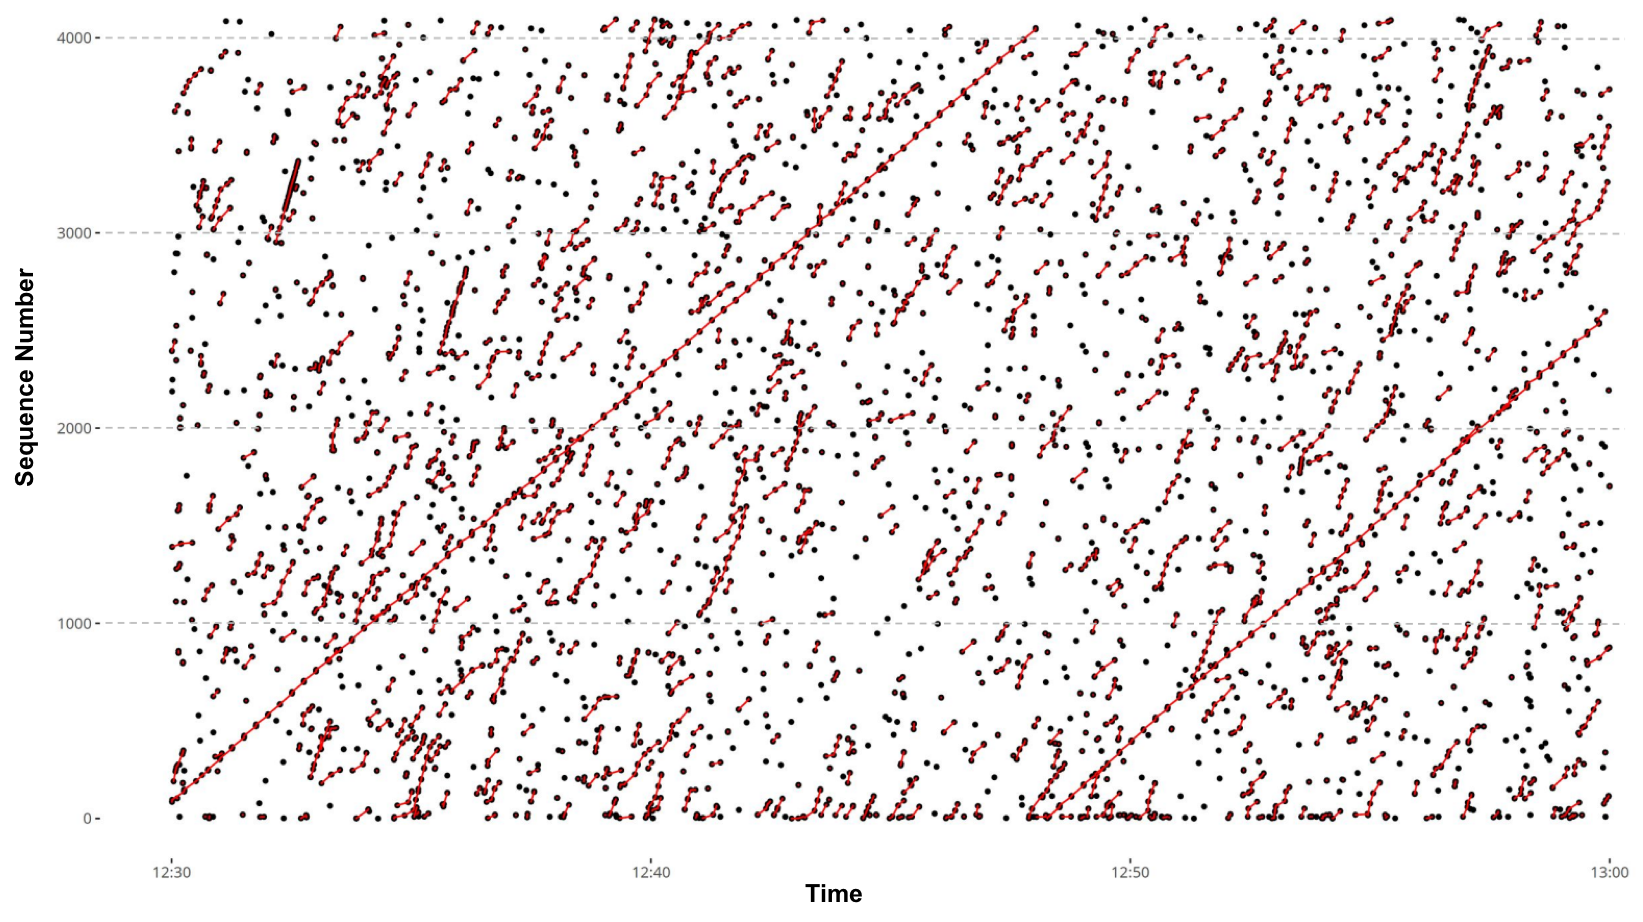
\includegraphics [width=\linewidth,trim=4 4 4 4,clip] {images/methodology_clustering.png}
		\caption{Clustering probe requests based on increasing sequence numbers present in them.}
		\label{clustering_pilot}
	\end{center}
\end{figure}


Figure \ref{clustering_pilot} shows the clustering process: 
the black dots show the probe requests and the red lines connect them into clusters representing those which were generated by the same device.
We finally combined both normal and anonymised probe requests, aggregated them based on their unique identifier, and removed repeating probe requests which reduced the difference between the sensor counts and the manual counts to -18\%.

\begin{figure}
	\begin{center}
		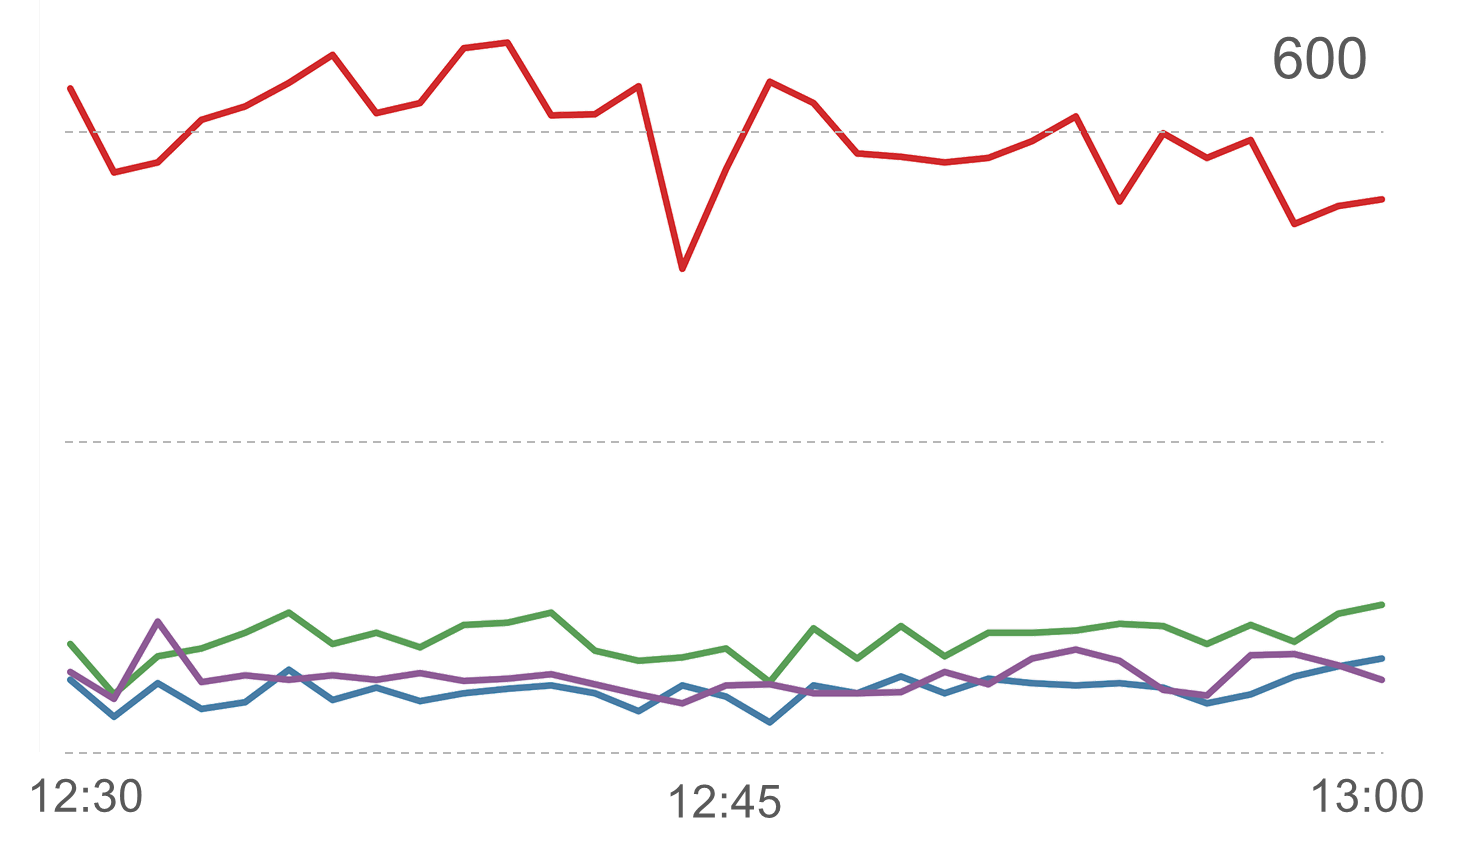
\includegraphics [width=\linewidth] {images/pilot_counts_comparision.png}
		\caption{Comparision of counts after filtering with manual counts}
		\label{comparision_pilot}
	\end{center}
\end{figure}
